\chapter{Pythia}
Pythia is a general-purpose event generator. It has been used for electron-positron and proton-proton collisions and for other physics studies. It is extensively used for studying physics at LHC. At the beginning the code was written in \verb+Fortran 77+, for the LHC era the experimental community made a decision to move the code to \verb!C++!. The latest version of Pythia (8.1) was released in 2007, which is written in \verb!C++! \citep{Buckley:2011ms}. 

In general Pythia performs on idea of the program designed here for the parton shower. However, it accounts for more of the underlying physics. 

\section{FastJet} 

\verb+FastJet+ is a \verb!C++! package provides a wide range of jet finding and analysis tools. It includes efficient implementation of all widely used sequential recombination jet algorithms for proton-proton ($pp$) and electron-positron ($ee^+$) collisions. In the case of jet clustering, the working principle is the same as the algorithm that we implemented in chapter 4, but it is much faster \citep{Buckley:2011ms}. 

In our work we generated 1000 events using Pythia 8.1 and analysed them using \verb+FastJet+. 

We extracted two observables the mass of the jet observable and the pseudo-mass observable. And also analysed some physical quantities, the transverse momentum $k_t$, pseudo-rapidity $\eta$ and the azimuth $\phi$. Here the value of the parameter $R$ is set to 1. For more about the documentation of \verb+FastJet+ see \citep{Buckley:2011ms}. 

\begin{figure}[hbtp]
\centering
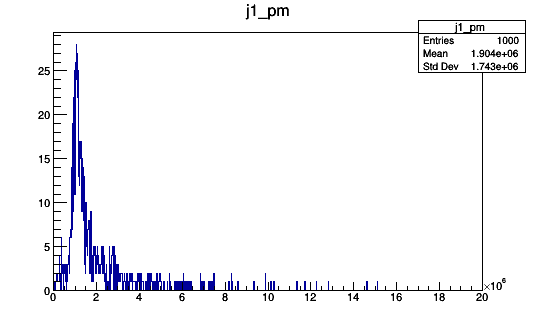
\includegraphics[scale=.7]{images/Canvas_1.png}
\caption{The pseudo-mass of jets obtained from analysing 1000 events. $R$ is chosen to be 1}
\end{figure}



\begin{figure}[hbtp]
\centering
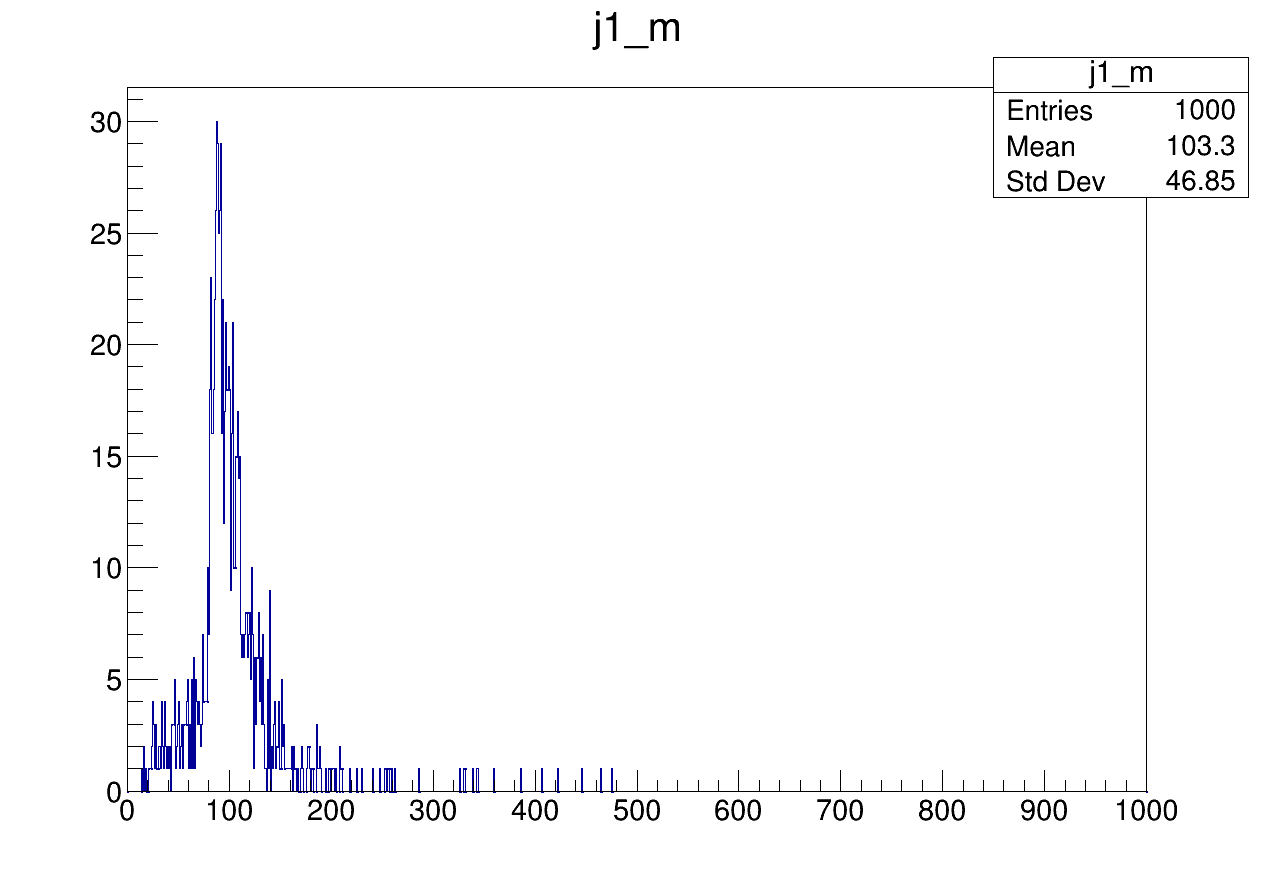
\includegraphics[scale=.3]{images/mass.png}
\caption{The mass of the jets obtained from analysing 1000 events.}
\end{figure}

 
\begin{figure}[hbtp]
\centering
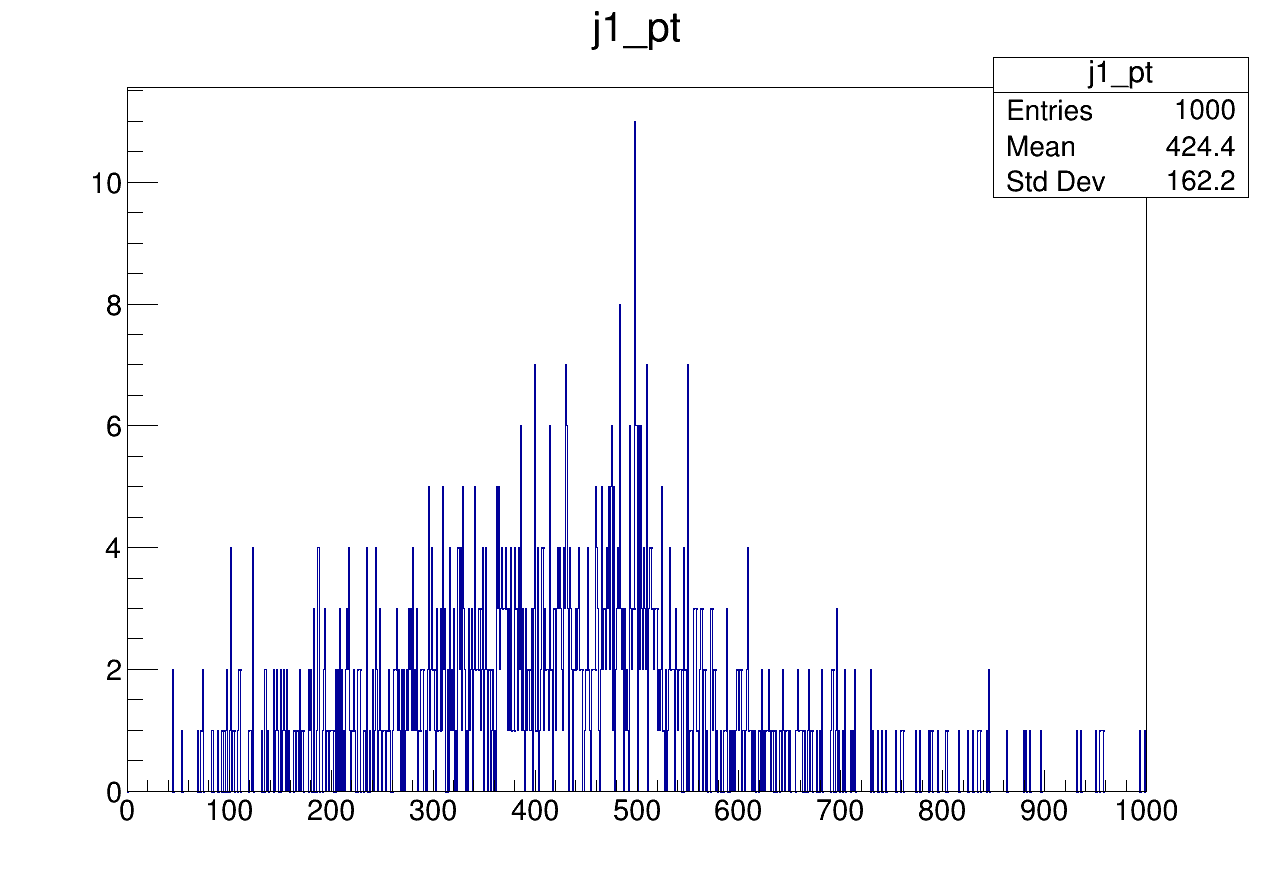
\includegraphics[scale=.3]{images/trnasverse.png}
\caption{The transverse momentum as it is obtained analysing from 1000 events.}
\end{figure}

\begin{figure}[hbtp]
\centering
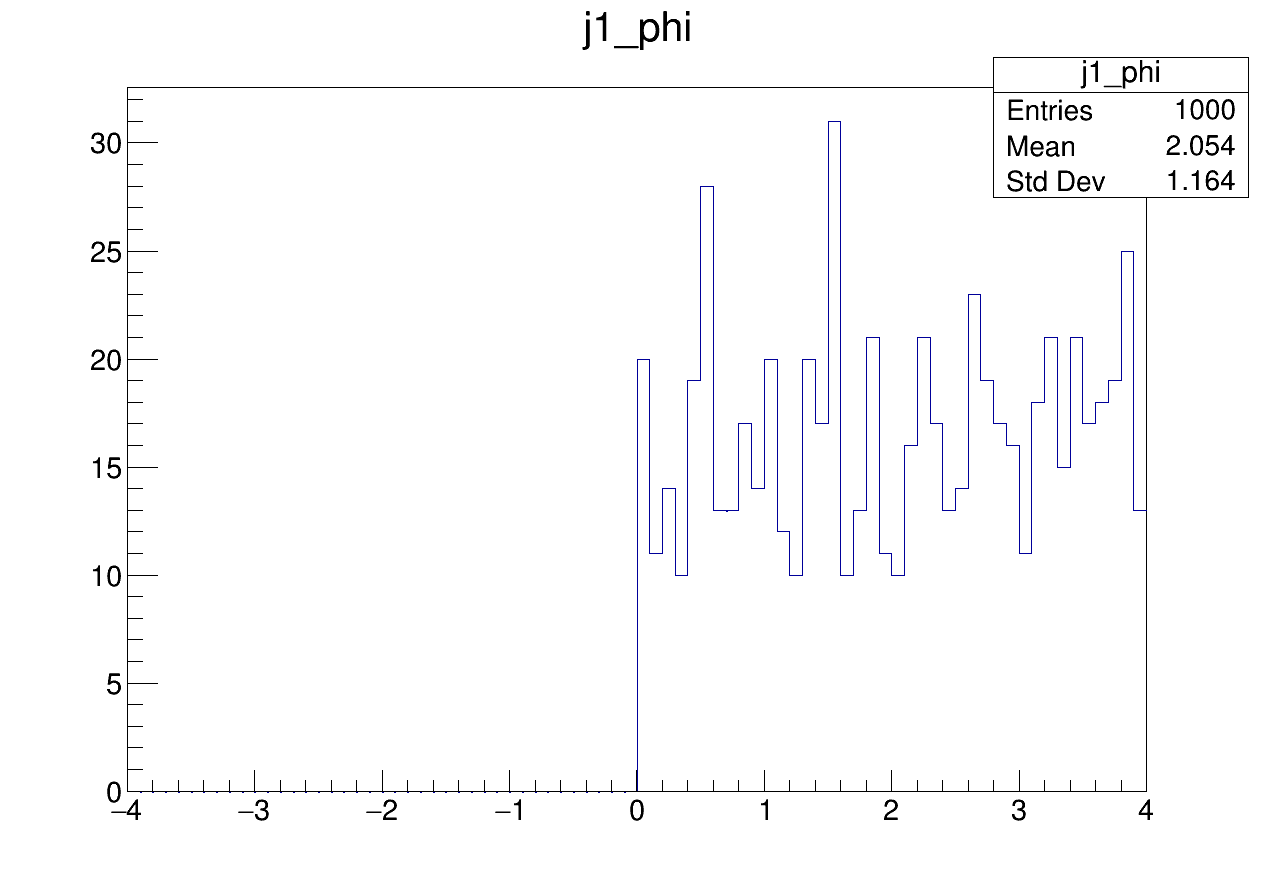
\includegraphics[scale=.4]{images/phi.png}
\caption{The Azimuth distance.  }
\end{figure}

\begin{figure}[hbtp]
\centering
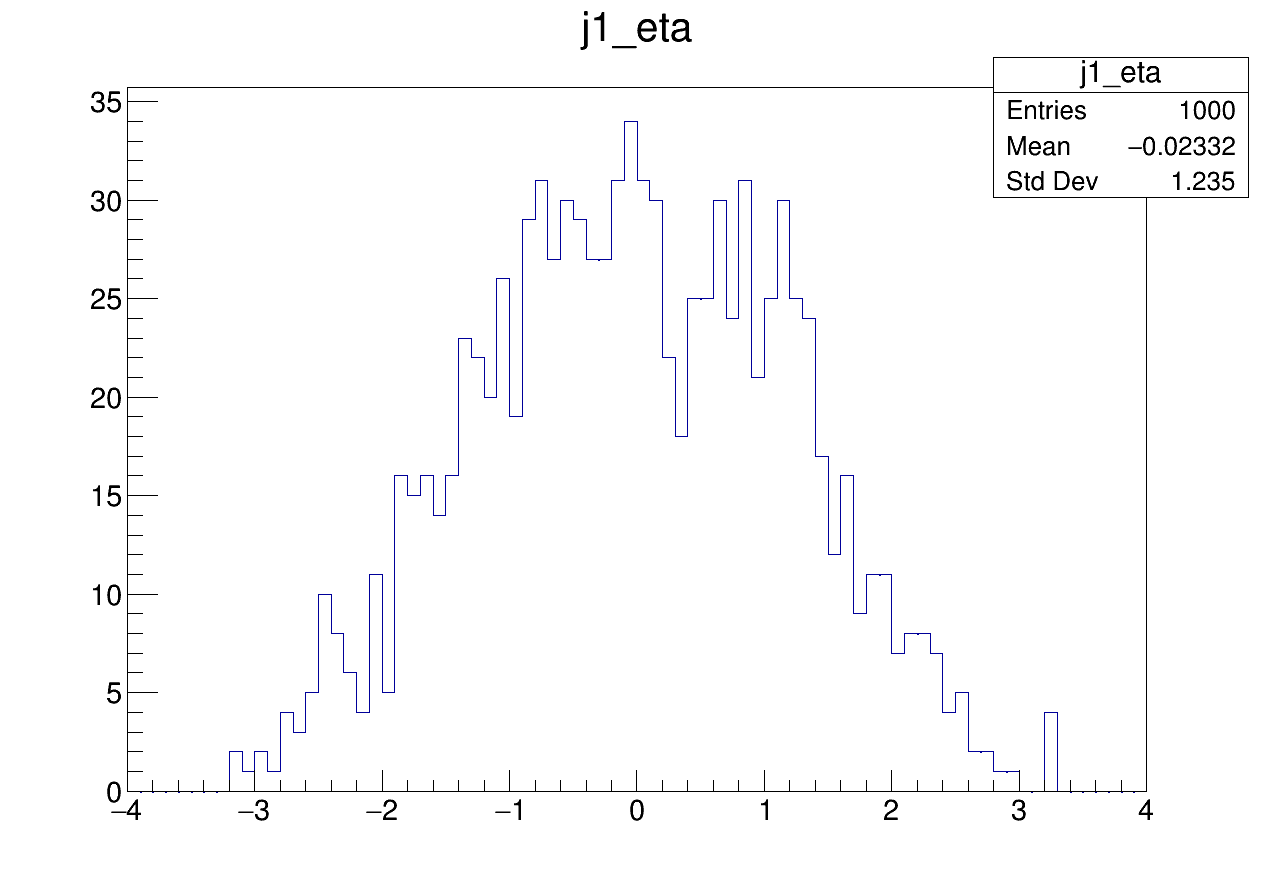
\includegraphics[scale=.3]{images/eta.png}
\caption{The pseudo-rapidity}
\end{figure}

      